\documentclass[a4paper,10pt]{article}
\usepackage{ucs}
\usepackage[utf8x]{inputenc}
\usepackage[dvips]{graphicx}
\usepackage{amsfonts}
\usepackage{appendix}
\usepackage[italian]{babel}

%opening
\title{Algoritmi euristici per la colorazione di grafi}
\author{Marco Pagliari\\matr 702501}

\newcommand{\tabucol}{\emph{Tabucol}}

\begin{document}
\maketitle

\begin{center}
Relazione progettuale per l'esame di Algoritmi Euristici
\end{center}

\vspace{2cm}

\begin{center}

\includegraphics[width=0.3\textwidth]{img/dtiLogo} 
\end{center}

\thispagestyle{empty}

\newpage

\tableofcontents
\listoffigures

\newpage

\begin{abstract}
Lo scopo del documento è di proporre una panoramica su alcune delle più note euristiche adottate per il problema della colorazione dei grafi, e più in dettaglio su: \emph{Simulated Annealing}, \emph{Tabu Search} e \emph{Variable Neighborhood Search}, tecniche che sono state direttamente implementate per studiarne le peculiarità ed analizzarne in pratica i risultati che permettono di ottenere, evidenziando come questo problema rimanga tutt'ora aperto a possibilità di miglioramento.
\end{abstract}

\section{Introduzione}
Il problema della colorazione di grafi è un famoso problema NP--difficile, ha numerose applicazioni pratiche come l'assegnamento di frequenze radio, la schedulazione di lavori nel tempo, l'allocazione di registri di un processore e la stampa di circuiti di test. Pur esistendo algoritmi esatti, che però sono in grado di risolvere istanze che non superino la soglia dei 100 vertici, diviene necessario ricorrere ad algoritmi euristici per risolvere istanze di grandi dimensioni. Le più recenti euristiche per la colorazione sono principalmente basate sullo schema della ricerca locale o su evoluzioni ibride di questa meta--euristica che combinano la semplice ricerca locale con metodi population--based.
Nel prosieguo del documento si introdurrà la descrizione formale del problema della colorazione di grafi, passando in breve rassegna le principali euristiche che sono state proposte nel corso degli anni, e analizzando in dettaglio tre fra queste tecniche con relativa descrizione delle caratteristiche implementative e dei risultati sperimentali ottenuti.

\section{Definizione del problema}
Dato un grafo $G=(V,E)$ con $V$ ed $E$ rappresentanti rispettivamente l'insieme dei vertici e l'insieme dei lati, e dato un numero intero $k$, una $k$--colorazione del grafo $G$ è una funzione del tipo: 

\begin{displaymath}
c:V\rightarrow\{1,\ldots,k\}\textrm{.}
\end{displaymath}

Il valore della funzione $c(x)$ di un vertice $x$ definisce il colore del vertice. Un insieme di vertici con lo stesso colore $i$ $(1\leq i \leq k)$ definisce una \emph{classe di colore}, che si denota con il simbolo $V_{i}$. Se due vertici adiacenti $x$ e $y$ sono colorati dello stesso colore $i$, tali vertici, il lato $[x,y]$ e il colore $i$ vengono detti \emph{in conflitto}. Una $k$--colorazione senza lati in conflitto viene definita \emph{legale}. Un insieme di vertici che non hanno nessun lato in comune viene detto \emph{insieme stabile}. Per quanto detto, una $k$--colorazione può essere definita legale se e solo se le sue classi di colori sono insiemi stabili. Il problema della colorazione di un grafo (Graph Coloring Problem, GCP) è quindi quello di determinare il più piccolo intero $k$, chiamato anche \emph{numero cromatico} del grafo $G$ e definito come $\chi(G)$, tale per cui esista una $k$--colorazione legale di $G$.

\begin{figure}[hp]
\begin{center}
 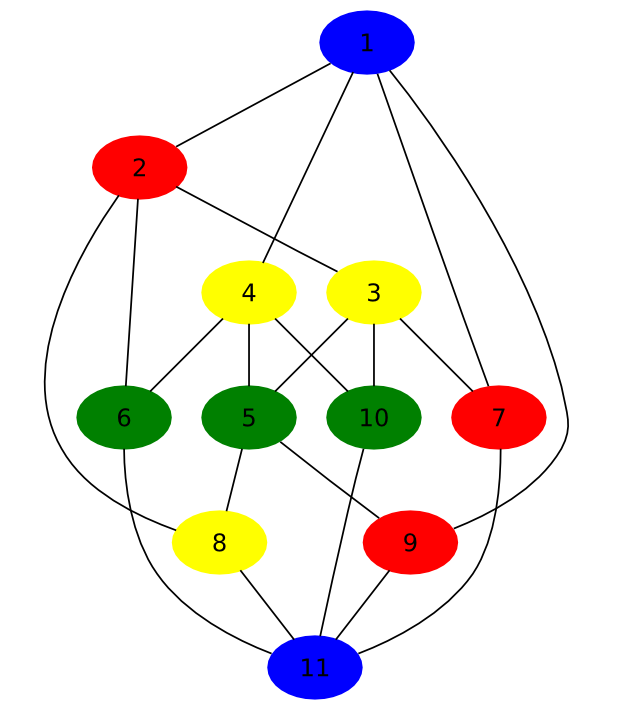
\includegraphics[width=0.5\textwidth]{img/ok}
\caption[Esempio di colorazione]{Esempio di $4$--colorazione legale per l'istanza DIMACS \emph{myciel3}, con 11 vertici e 20 lati. Per questa istanza, inoltre, il numero cromatico del grafo è pari a $4$, per cui la figura esprime una colorazione minima.}
\end{center}
\end{figure}

\begin{figure}[hp]
\begin{center}
 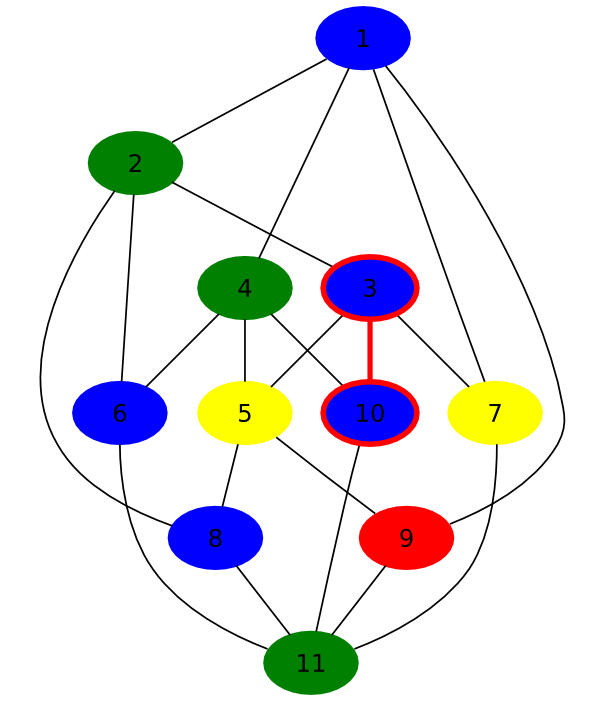
\includegraphics[width=0.5\textwidth]{img/err}
\caption[Esempio di colorazione]{Esempio di $4$--colorazione non legale per l'istanza DIMACS \emph{myciel3}. Sono stati evidenziati i nodi 3 e 10 e il lato che li collega, per mostrare cosa si intende per conflitto: essi infatti appartengono alla medesima classe colore e sono vertici adiacenti, per cui si dicono in conflitto.}
\end{center}
\end{figure}

Dato un intero $k$, il problema della ricerca dell'esistenza di una $k$--colorazione legale di $G$ viene anche chiamato $k$--GCP. Un algoritmo di ricerca locale per il GCP può essere utilizzato per risovere il $k$--GCP, semplicemente fermando la ricerca nel momento in cui una colorazione legale viene trovata. Inoltre, un algoritmo che risolve il $k$--GCP può essere naturalmente utilizzato per risolvere il GCP, seguendo questi passi:

\begin{enumerate}
\item Determinare una colorazione legale $c$ attraverso un algoritmo \emph{greedy}.
\item Impostare $k^{*}$  pari al numero di colori utilizzati in $c$ e $k=k^{*}-1$.
\item Risolvere il $k$--GCP e se viene trovata una valida $k$--colorazione ritornare al passo 2, altrimenti restituire $k^{*}$.
\end{enumerate}

Anche se potrebbe sembrare che, con questa metodologia, si possa spendere tempo nel trovare $k$--colorazioni legali con valori non minimi di $k$, in realtà la maggior parte del tempo computazionale verrà spesa nel trovare una $k^{*}$--colorazione legale e nel tentare, senza successo, di trovare una $(k^{*}-1)$--colorazione, in quanto il tempo computazionale impiegato dall'algoritmo generalmente aumenta in modo esponenziale al diminuire del numero di colori richiesto per la colorazione: per questo motivo saranno proprio le ultime iterazioni ad incidere in modo significativo sul valore complessivo del tempo impiegato per trovare una colorazione minima. Sarebbe in alternativa possibile utilizzare un approccio inverso, in cui il $k$--GCP viene risolto con $k$ progressivamente maggiore, tuttavia questo approccio non è raccomandabile, in quanto spreca gran parte del tempo di elaborazione a ricercare $k$--colorazioni con $k<\chi(G)$.

\section{Approcci dalla letteratura}
Esistono differenti approcci proposti per risolvere il problema: di seguito se ne propone un brevissimo accenno rispetto agli autori e alle euristiche che hanno utilizzato.

\begin{description}
\item[Chams et al. (1987)] Si pongono come obiettivo il minimizzare il numero di lati in conflitto attraverso il cambiamento del colore di un singolo vertice della soluzione, mediante l'utilizzo della meta--euristica del \emph{Simulated Annealing}.

\item[Hertz and de Werra (1987).] Applicano la meta--euristica del \emph{Tabu Search} proposta da Glover \cite{tabusearch}, per definire quella che viene riconosciuta come l'implementazione classica del \tabucol{}.

\item[Johnson et al. (1991).] Confrontano tre differenti algoritmi che utilizzano il \emph{Simulated Annealing} con diverse strategie di ricerca:
\begin{itemize}
 \item Soluzioni non necessariamente legali con un numero non fisso di classi di colore.
 \item Soluzioni legali con un numero di classi di colore non fisso.
 \item Soluzioni non necessariamente legali con penalità. 
\end{itemize}

\item[Davis (1991).] Implementano con scarso successo il primo algoritmo genetico che fonde permutazioni di vertici colorati in modo greedy.

\item[Costa et al. (1995).] Attraverso una ricerca locale genetica, propongono una popolazione di soluzioni su cui lavorare attraverso un algoritmo di discesa locale e un operatore di crossover.

\item[Mladenovic and Hansen (1997).] Applicano la tecnica del \emph{Variable Neighborhood Search} per la colorazione dei grafi, proponendo ben 11 differenti intorni, più o meno redditizi, e utilizzando l'algoritmo \tabucol{} per discendere localmente nello spazio delle soluzioni. Si differenzia rispetto alla recente corrente di algoritmi ibridi proposti per la risoluzione del problema di colorazione.

\item[Galinier and Hao (1999).] Implementano un altro algoritmo di ricerca locale genetica, sfruttando il \tabucol{} per gestire la variabilità della popolazione e un operatore di crossover che ricombina le classi colore: è una delle tecniche che hanno permesso di ottenere i risultati migliori.
\end{description}

\section{Euristiche Implementate}
\subsection{Tabu Search}
\subsubsection{Approccio teorico}
Uno dei primi metodi di ricerca che sono stati proposti per la colorazione di un grafo è l'algoritmo \tabucol{}  \cite{tabucol}, sviluppato nel 1986 e pubblicato nel 1987, un anno dopo la pubblicazione del documento di Fred Glover \cite{tabusearch} che ha introdotto l'euristica del \emph{Tabu Search}. Originariamente sviluppato da Hertz e de Werra, l'algoritmo \tabucol, pur essendo conosciuto da ben 20 anni, è ancora frequentemente utilizzato, nella sua versione classica piuttosto che nelle varie versioni migliorate proposte nel corso degli anni\cite{tabucolimproved}, come subroutine di ricerca locale in numerosi algoritmi ibridi.

Il \tabucol{} è un algoritmo di tabu--search per il $k$--GCP: inizialmente esso prevede la generazione di una soluzione casuale, la quale tipicamente contiene un elevato numero di spigoli in conflitto. A partire da questo stato, l'euristica modifica ad ogni iterazione la colorazione di un singolo vertice, con l'obiettivo di diminuire progressivamente il numero di spigoli in conflitto fino ad ottenere, ove possibile, una $k$--colorazione legale. A questo scopo viene utilizzata una lista tabu che permette di fuoriuscire da zone di ottimo locale.

\tabucol{} effettua l'esplorazione dello spazio $S$ delle soluzioni, che è costituito dall'insieme di tutte le possibili $k$--colorazioni del grafo $G$ assegnato. Una soluzione $c\in S$ viene considerata una partizione dell'insieme $V$ dei vertici in $k$ sottoinsiemi $V_{1},\ldots,V_{k}$. La funzione di valutazione $f$ misura il numero di spigoli in conflitto, per cui per una soluzione $c=(V_{1},\ldots,V_{k})$ contenuta in $S$, la funzione obiettivo si prefiggerà di minimizzare la seguente:
\begin{displaymath}
f(c)=\sum_{i=1}^{k}|E_{i}|, 
\end{displaymath}
dove $E_{i}$ identifica l'insieme di spigoli in conflitto che insistono sulla stessa classe di colore $V_{i}$. L'obiettivo dell'algoritmo è di determinare una $k$--colorazione $c$ legale, quindi tale per cui sia $f(c)=0$. 

Una trasformazione elementare, chiamata \emph{$1$--mossa}, consiste nel cambiare il colore di un singolo vertice: per un vertice $v$ e un colore $i\neq c(v)$, si può definire una $1$--mossa come la coppia $(v,i)$ che assegna il colore $i$ al vertice $v$, il che implica che la soluzione risultante dalla $1$--mossa possa essere definita dall'operazione $c+(v,i)$. 
\pagebreak
La $k$--colorazione $c'=c+(v,i)$ può quindi essere descritta in questo modo:
\begin{itemize}
 \item $c'(v)=i$\textrm{.}
 \item $c'(w)=c(w) \quad \forall w \in V-\{v\}$\textrm{.}
\end{itemize}
L'intorno $N(c)$ di una soluzione $c\in S$ viene definito come l'insieme delle $k$--colorazioni che possono essere raggiunte da quella corrente $c$ attraverso l'applicazione di una $1$--mossa. Per questo l'intorno conterrà $|V|(k-1)$ soluzioni. I benefici apportati da una $1$--mossa $(v,i)$ possono essere misurati dalla funzione profitto $\delta(v,i)=f(c+(v,i))-f(c)$. Un valore negativo della funzione $\delta(v,i)$ indicherà che la $1$--mossa implica una diminuizione della funzione obiettivo.

Estremamente importante per l'algoritmo è la nozione di \emph{vertici in conflitto}: è possibile indicare con $F(c)$ il numero dei vertici in conflitto per la colorazione corrente $c$. Una $1$--mossa $(v,i)$ che coinvolge un vertice in conflitto viene detta \emph{critica}. Per motivi di efficienza, l'algoritmo \tabucol{} realizza soltanto $1$--mosse critiche.

La lista tabu, all'interno dell'algoritmo, svolge il ruolo di salvare le mosse effettuate. Quando viene realizzata una $1$--mossa $(v,i)$ su una soluzione $c$, viene salvata nella lista la coppia $(v,c(v))$, che significa che è proibito riassegnare il colore $c(v)$ al vertice $v$ per un certo numero di iterazioni. La durata dello stato di tabu della $1$--mossa $(v,c(v))$ dipende dal numero dei vertici in conflitto in $c$ e da due parametri configurabili: $L$ e $\lambda$. In modo più preciso, quando viene applicata alla soluzione corrente una determinata $1$--mossa, la coppia $(v,c(v))$ diventa tabu per un numero $L+ \lambda F(c)$ di iterazioni. Una $1$--mossa viene definita \emph{candidata} se è sia critica che non tabu o se soddisfa il criterio di aspirazione, il quale nell'implementazione originaria era semplicemente $f(c+(v,i))=0$, cioè se l'ignorare il fatto che la mossa sia tabu porta ad una $k$--colorazione legale. In questa versione dell'algoritmo è stato deciso di utilizzare un criterio di aspirazione meno stringente e di considerare la mossa come non tabu qualora porti ad un miglioramento rispetto all'ottimo globale fino a quel momento trovato.

Ad ogni iterazione l'algoritmo effettua la migliore $1$--mossa candidata, fermandosi quando $f(c)=0$ e ritornando la $k$--colorazione $c$ legale del grafo $G$ passato per argomento.

Lo pseudocodice dell'algoritmo è il seguente:

\begin{quote}
\textbf{Euristica di Tabu Search:}

Input: Un grafo $G=(V,E)$, e un intero $k>0$. \\
Paramerti: \emph{MaxIter}, $L$ and $\lambda$. \\
Output: La soluzione $c^{*}$.

Costruisci una soluzione casuale $c$. \\
Imposta $c^{*}=c$ e $iter=0$. \\
Crea la lista tabu e impostala in modo che nessuna mossa sia tabu.

Ripeti fino a che $f(c)==0$ oppure $iter==MaxIter$:

\hspace*{8pt}Imposta $iter=iter+1$. \\
\hspace*{8pt}Scegli $1$--mossa $(v,i)$ candidata con $\delta(v,i)$ minima. \\
\hspace*{8pt}Inserisci $(v,c(v))$ nella lista tabu per $L+\lambda F(c)$ iterazioni. \\
\hspace*{8pt}Imposta $c=c+(v,i)$; se $f(c)<f(c^{*})$ allora $c^{*}=c$ e \emph{iter=0}.

\end{quote}

\subsubsection{Approccio implementativo}
\begin{description}
 \item[Soluzione iniziale.] La soluzione iniziale viene costruita nel modo più semplice: in modo casuale. Una alternativa consiste nel costruire una soluzione attraverso un'algoritmo \emph{greedy}, che però non sembra dare tangibili vantaggi per la maggior parte dei grafi.

\item[$1$--Mosse critiche.] L'algoritmo \tabucol{} considera soltanto $1$--mosse $(v,i)$ in cui $v$ è un vertice in conflitto, il che permette di guidare la ricerca attraverso regioni dello spazio delle soluzioni più appetibili. Come si può notare nell'esecuzione, la funzione obiettivo diminuisce rapidamente nelle prime fasi della ricerca e l'euristica impiega la maggior parte del tempo computazionale ad eliminare gli ultimi lati in conflitto.

\item[Intorno completo.] La ricerca della migliore $1$--mossa realizzata ad ogni iterazione è la migliore fra tutte le $1$--mosse critiche. 

\item[Criterio di aspirazione.] A differenza della classica implementazione dell'algoritmo in cui lo stato di tabu di una $1$--mossa veniva ignorato nel caso questa potesse portare ad una colorazione legale, si è deciso di utilizzare un criterio meno stringente, che ignora lo stato tabu di una certa mossa qualora il risultato che essa porterebbe è migliore dell'ottimo risultato trovato fino a quel punto.

\item[Durata tabu.] Il numero di $1$--mosse critiche è proporzionale al numero di vertici in conflitto e può variare in modo dinamico durante il processo di ricerca. Anche se esistono diverse opinioni secondo la configurazione dei parametri $L$ e $\lambda$, questi dipendono sempre dalla tipologia di istanze affrontate: per questo non si può dire quale dei metodi possa essere il migliore, ma idealmente questi due parametri dovranno essere configurati istanza per istanza. Per le prove sperimentali effettuate si è valutato che i migliori risultati si sono ottenuti impostanto $10<L<20$ e $\lambda=0.6$.

\item[Strutture dati.] La maggior parte del tempo computazionale viene speso ad ogni iterazione per scegliere la migliore $1$--mossa critica. Una implementazione efficiente permette di ridurre notevolmente la complessità dell'algoritmo. Sia $\gamma(v,i)$ il numero di vertici adiacenti a $v$ ed aventi il colore $i$ nella soluzione corrente $c$ e si assuma che che questi valori siano salvati in una matrice $|V|\times k$ delle adiacenze, chiamata $\gamma$--matrice. La matrice delle adiacenze dovrà essere inizializzata all'inizio del processo di ricerca e successivamente aggiornata ad ogni iterazione quando una $1$--mossa viene effettuata per modificare la soluzione $c$.

Calcolare il profitto di una $1$--mossa può ridursi a complessità costante, data dall'operazione $\delta(v,i)=\gamma(v,i)-\gamma(v,c(v))$. E' inoltre possibile determinare in tempo costante se un vertice sia in conflitto, consultando la matrice di adiacenza e verificando che $\delta(v,c(v))>0$. Per trovare la migliore $1$--mossa è sufficiente effettuare una ricerca all'interno della $\gamma$--matrice in tempo $O(kF(c))$. Muovendosi da una soluzione $c$ ad una $c+(v,i)$, è possibile aggiornare la matrice delle adiacenze in tempo $O(|\Gamma(v)|)$, dove $\Gamma(v)$ rappresenta l'insieme dei vertici adiacenti a $v$: per ogni vertice $w\in \Gamma(v)$, è sufficiente incrementare $\delta(w,i)$ di un'unità e diminuire $\delta(w,c(v))$ di un'unità. Per questo ogni iterazione richiede in termini computazionali $O(\min \{kF(c),|\Gamma(v)|\})$.

La lista tabu viene invece salvata all'interno di un'altra matrice $T$ $(|V|\times k)$, dove $T(v,i)$ rappresenta l'iterazione in cui la $1$--mossa cesserà di essere tabu. Attraverso questa struttura è possibile conoscere in tempo costante se una data $1$--mossa è tabu e aggiornare la matrice stessa, in seguito ad una mossa, impostando $T(v,i) =iter+L+\lambda F(c)$.

\item[Intensificazione e diversificazione.] Benchè siano state proposte dallo stesso Glover, l'ideatore della ricerca tabu, nell'algoritmo \tabucol{} non sono state introdotte ulteriori tecniche di intensificazione e diversificazione, se non quella intrinseca nel meccanismo di impostazione della durata tabu, che dipende dinamicamente dal valore della funzione obiettivo attuale.

\item[Condizione di terminazione.] Anzichè fissare un valore statico in cui far terminare l'esecuzione dell'algoritmo, è sembrato conveniente invece impostare un limite massimo di iterazioni possibili senza miglioramento della soluzione corrente. In questo modo si è in grado di controllare in modo più raffinato l'esecuzione dell'algoritmo, e la sua discesa verso l'ottimo, anche se potenzialmente ci si espone al problema di prolungarne l'esecuzione per un tempo non bene definito, seppur comunque limitato.

\item[Miglioramento: colorazione casuale nodi in conflitto.] Durante le prove sperimentali è stato testata una variazione della classica implementazione del \tabucol{}, che prevede di ridurre notevolmente il numero di iterazioni massime a cui far terminare l'algoritmo, richiamandolo come subroutine in modo iterativo, alternato con una colorazione casuale dei restanti nodi in conflitto. Come si vedrà nel capitolo dedicato alle prove sperimentali, questo ha permesso di ottenere risultati incoraggianti dove invece il normale \tabucol{} non era in grado di fuoriuscire da zone di ottimo locale in breve tempo.
\end{description}

\subsection{Simulated Annealing}
\subsubsection{Approccio Teorico}
L'euristica dell'annichilazione simulata prende il nome dall'analogia che stabilisce con il processo fisico sfruttato nella tecnica metallurgica per aumentare le dimensioni dei cristalli di un materiale riducendone i difetti, attraverso il riscaldamento e un successivo raffreddamento controllato dello stesso. Il riscaldamento permette agli atomi che lo compongono di liberarsi da parte dei legami che li mantengono fissi all'interno di uno schema rigido nella posizione di partenza (un minimo locale di energia interna) e muoversi più liberamente all'interno del materiale. Il lento raffreddamento fa si che vi siano maggior possibilità di trovare configurazioni con una più bassa energia interna rispetto a quella iniziale.
Analogamente l'euristica di \emph{annichilazione simulata} procede sostituendo alla soluzione iniziale una soluzione vicina scelta casualmente nell'intorno con una probabilità che dipende dalla variazione introdotta nella funzione obiettivo e da un valore di temperatura che viene gradualmente fatto diminuire. Più precisamente, se il cambiamento introdotto provoca un miglioramento della funzione obiettivo questo viene sempre effettuato, mentre se il cambiamento è peggiorante allora viene deciso di metterlo in pratica solo con una specifica probabilità dipendente dal rapporto fra peggioramento e valore corrente della temperatura. In pratica il processo di movimento da una soluzione alla successiva segue le seguenti regole:

\begin{itemize}
 \item Scelta di una soluzione casuale $x$ compresa nell'intorno di quella corrente $x^{*}$:
\begin{itemize}
 \item La nuova soluzione viene accettata se è migliore di quella corrente, cioè se $f(x)\leq f(x^{*})$.
 \item Se la nuova soluzione è invece peggiore di quella corrente, cioè se $f(x)>f(x^{*})$, allora questa viene accettata soltanto se il valore $r$ generato casualmente nell'intervallo $[0,1]$ risulta essere:
\begin{displaymath}
 r<e^{(f(x^{*})-f(x))/T^{(k)}}\textrm{.}
\end{displaymath}
\end{itemize}
\end{itemize}

L'accettazione di mosse peggioranti permette all'algoritmo di evadere da zone di ottimo locale nel momento in cui la temperatura del sistema abbia un valore tale da permetterlo: più la temperatura è elevata più sarà semplice per l'algoritmo accettare mosse peggioranti, più la temperatura si avvicina allo zero, più sarà improbabile che l'algoritmo accetti di eseguire una mossa peggiorante.

L'euristica di annichilazione simulata proposta Kirkpatrick et al.\cite{sa} per simulare un insieme di atomi in ricerca di equilibrio è stata successivamente  ripresa da Hertz e de Werra\cite{sa_hertz_dewerra} per applicarla al problema della colorazione dei grafi. Secondo quanto proposto l'algoritmo parte generando casualmente una colorazione iniziale non ammissibile estraendo iterativamente una serie di soluzioni vicine mediante la diversa colorazione di un nodo conflittuale, cercando di raggiungere una soluzione ottima. 

In una procedura di annichilazione simulata la temperatura viene impostata inizialmente ad un valore arbitrariamente elevato e viene diminuito gradualmente, nel seguente modo:

\begin{displaymath}
 T^{(k+1)}=\sigma \cdot T^{(k)},
\end{displaymath}

dove $\sigma$ rappresenta il fattore di raffreddamento, in modo che la probabilità di accettare peggioramenti alla soluzione diminuisca parallelamente al raffreddarsi del sistema. Questo in teoria dovrebbe consentire inizialmente all'algoritmo di privilegiare la diversificazione esplorando ampie regioni dello spazio delle soluzioni e al ridursi della temperatura di intensificare sempre più, cercando di trovare la soluzione ottima in una ristretta, ma più dettagliatamente analizzata, regione dello spazio delle soluzioni.

L'approccio scelto in questo caso è lo stesso utilizzato nel caso precedente con l'euristica del tabu search, ovvero quello di minimizzare il numero di nodi in conflitto in una colorazione non necessariamente legale con numero di classi colore fissato.
Dato un grafo $G=(V,E)$ e un numero di colori $k$, vengono considerate come soluzioni le partizioni di $V$ in $k$ insiemi, e la funzione obiettivo prevede di minimizzare il numero di nodi in conflitto (o in modo equivalente di lati in conflitto). Una partizione $\Pi_{2}$ è compresa nell'intorno della partizione $\Pi_{1}$ (e quindi ne costituisce un valido vicino) se queste differiscono soltanto per la posizione di un singolo vertice $v$ conflittuale in $\Pi_{1}$. Si noti che questa definizione di intorno non è simmetrica: in particolare una colorazione legale non ha un intorno in quanto non contiene nodi in conflitto.

Lo pseudocodice dell'algoritmo è il seguente:

\begin{quote}
\textbf{Euristica Simulated Annealing:}

Input: Un grafo $G=(V,E)$, e un intero $k>0$.\\
Paramerti: $T$, $T_{min}$, $\sigma$ e $MaxIter$.\\
Output: La soluzione $c^{*}$.

Costruisci una soluzione casuale $c$.\\
Imposta $c^{*}=c$ e $iter=0$.

Ripeti fino a che $f(c)==0$ oppure $T\leq T_{min}$:

\hspace*{8pt}Ripeti fino a $f(c)==0$ oppure $iter > MaxIter$:

\hspace*{16pt}Scegli una $1$--mossa $(v,i)$ casuale fra i nodi conflittuali.\\
\hspace*{16pt}Sia $f(c)$ il costo della nuova soluzione $c$, calcola $\Delta=f(c^{*})-f(c)$.

\hspace*{16pt}Se $\Delta > 0$ allora:\\
\hspace*{24pt}Imposta $c^{*}=c$ e $iter=0$.\\
\hspace*{16pt}Altrimenti:\\
\hspace*{24pt}Imposta $iter=iter+1$.\\
\hspace*{24pt}Genera un numero casuale $r$ compreso nell'intervallo [0,1].\\
\hspace*{24pt}Se $r\leq e^{\Delta/T}$ allora imposta $c^{*}=c$.

\hspace*{8pt}Decrementa il valore di temperatura $T=\sigma \cdot T$.\\
\hspace*{8pt}Reimposta $iter=0$.

\end{quote}

\subsubsection{Approccio Implementativo}
Un algoritmo di ricerca locale basato su un intorno con $k$ fissato può essere semplicemente implementato attraverso l'estrazione casuale di una $1$--mossa all'interno dell'insieme dei nodi in conflitto per tutte le possibili diverse colorazioni che il nodo estratto può assumere. 
Anche in questa implementazione si è scelto di utilizzare la $\gamma$--matrice di adiacenza utilizzata per il Tabu Search, in modo da riuscire ad ottenere rapidamente il profitto $\delta(v,i)$ introdotto da una determinata mossa e calcolare la conseguente variazione nella funzione obiettivo. 

\begin{description}
 \item[Scelta dei livelli di temperatura.] Per ottenere buoni risultati con questa euristica, risulta necessario dedicare grande attenzione alla taratura dei parametri relativi alla temperatura. Dopo numerose prove sperimentali si è rilevato che la scelta di impostare la temperatura iniziale $T^{(0)}$ come la distanza della più lontana soluzione appartenente all'intorno di quella iniziale (equivalente al grado di adiacenza massimo per i nodi del grafo) fosse inutilmente dispendiosa per istanze complesse come quelle prese in considerazione per i test, che possono presentare nodi con grado elevato. Per questo motivo si è scelto di lasciare il parametro configurabile per ogni specifica istanza, anche se si sono ottenuti risultati soddisfacenti per un valore intorno a $3.5$.

Secondo importante parametro da configurare è il fattore $\sigma$ di riduzione della temperatura, che permette di decidere l'accuratezza dell'algoritmo, ma allo stesso tempo va ad incidere fortemente sulle prestazioni dello stesso. Per questo è importante raggiungere un buon compromesso fra le prestazioni che si attendono dall'algoritmo e i risultati che si vogliono raggiungere. Per le prove sperimentali che sono state effettuate si è ottenuto il miglior rapporto risultati/prestazioni con $\sigma=0.9999$.

Terzo parametro è quello della temperatura finale $T_{min}$ del sistema, a cui si vuole far terminare la ricerca dell'algoritmo. Sempre dopo la campagna di test sperimentali si è scelto di impostare il valore intorno a $T_{min}=0.01$, in quanto impostare il parametro a valori inferiori non andava a beneficio della bontà dei risultati dell'algoritmo, ma ne allungava soltanto i tempi di esecuzione.

\item[Scelta del numero di iterazioni a temperatura costante.]In questa implementazione dell'euristica del Simulated Annealing si è deciso di far effettuare all'algoritmo una serie di iterazioni a temperatura costante. L'algoritmo è stato tarato per effettuare $n$ estrazioni senza miglioramenti, a temperatura costante. Nel caso di miglioramenti il contatore viene azzerato e si procede alla stessa temperatura fino a che non vengono effettuate $n$ iterazioni senza incontrare un miglioramento nella soluzione attuale.

Si è notato dalle prove sperimentali che lasciando questo parametro costante non si riusciva ad ottenere un buon compromesso fra prestazioni e risultati, in quanto troppe iterazioni a temperature elevate risultano spesso uno spreco di risorse, mentre sarebbe stato più utile dedicare più tempo computazionale a bassi livelli di temperatura, quando l'algoritmo si occupa di intensificare la soluzione. Per questo si è scelto di far variare il numero delle iterazioni a temperatura costante in modo inversamente proporzionale all'andamento della temperatura, così da far aumentare il numero di iterazioni al decrescere della temperatura. In questo modo è stato possibile dedicare minore tempo a livelli di temperatura elevata e incentrare la maggior parte del tempo di elaborazione nelle fasi di intensificazione in cui la temperatura del sistema scende al di sotto del valore $T=1$. Per evitare naturalmente che il numero di iterazioni a temperatura costante tenda all'infinito, si è scelto di imporre un valore massimo, sperimentalmente fissato intorno a $100$.
\end{description}

\subsection{Variable Neighborhood Search}
\subsubsection{Approccio Teorico}
Hansen e Mladenovic hanno proposto \cite{vns} nel 1997 il metodo di ricerca ad intorno variabile, che consiste nel modificare sistematicamente l'intorno durante la ricerca della soluzione ottima. L'euristica, a differenza della quasi totalità di quelle basate sulla classica ricerca locale, non segue una traiettoria ben definita, ma esplora intorni della soluzione corrente progressivamente più distanti attraverso la generazione di nuove soluzioni casuali, muovendosi verso queste soltanto se si realizza un miglioramento. Successivamente a questo movimento, viene aplicata ripetutamente una routine di ricerca locale per discendere nell'ottimo locale dell'intorno. 

Sia $S$ l'insieme delle soluzioni di un problema di ottimizzazione combinatoria, per una soluzione $s_{i} \in S$, venga indicato con $N(s_{i})$ l'intorno di $s_{i}$, definito come l'insieme delle soluzioni vicine a $s_{i}$ attraverso l'attuazione di una modifica locale. L'idea che stà alla base del Variable Neighborhood Search consiste nell'utilizzare differenti intorni durante la ricerca: data la soluzione corrente $s$, una soluzione vicina $s'$ viene generata attraverso le regole stabilite per l'intorno selezionato e successivamente viene applicata una subroutine di ricerca locale a $s'$ in modo da discendere verso l'ottimo locale $s''$. Nel caso che $s''$  sia migliore di $s$, allora questa diventerà la nuova soluzione corrente, altrimenti viene considerato un nuovo intorno per cercare di migliorare $s$. Il processo viene ripetuto fino a che nessun intorno porta ad un miglioramento. 

L'euristica VNS è stato applicata nel 2003 da Avanthay, Hertz e Zufferey \cite{vns_hertz} al problema della colorazione dei grafi: come per le due euristiche precedenti si è scelto di seguire l'approccio del partizionamento in classi di colore del grafo, quindi di porsi come funzione obiettivo la minimizzazione di nodi (o lati) in conflitto, come si può vedere dal seguente pseudocodice:

\begin{quote}
\textbf{Euristica Variable Neighborhood Search:}

Input: Un grafo $G=(V,E)$, e un intero $k>0$.\\
Paramerti: \# intorni\footnote{In questa implementazione è pari a 5.} \\
Output: La soluzione $c^{*}$.

Costruisci una soluzione casuale $c$.\\
Imposta $c^{*}=c$, $iter=0$ e $t=1$.

Ripeti fino a che $f(c)==0$ oppure $iter=|V|$:

\hspace*{8pt}\emph{Shaking}. Genera $s'$ dall $t$--esimo intorno di $s$ ($s' \in N^{(t)}(s)$).

\hspace*{8pt}\emph{Ricerca Locale}. Applica a $s'$ una subroutine di ricerca locale\\ 
\hspace*{78pt}e sia $s''$ l'ottimo locale trovato.

\hspace*{8pt}\emph{Muovi o no}. Se $s''$ è migliore di $s$ allora:\\
\hspace*{16pt}Imposta $s=s''$, $t=1$ e $iter=0$.\\
\hspace*{16pt}Altrimenti incrementa $iter$, e $t$ se $iter$ è multiplo di $\lceil\frac{|V|}{5}\rceil$.
\end{quote}

L'euristica, a partire da una soluzione iniziale generata in modo casuale, esplora lo spazio delle soluzioni utilizzando una permutazione dei differenti intorni a disposizione, discendendo verso l'ottimo locale della nuova soluzione estratta e vi si muove solo se migliorante rispetto a quella corrente.

\subsubsection{Approccio Implementativo}
Generando la soluzione iniziale in modo casuale si fermerà l'algoritmo dopo che $|V|$ iterazioni sono state effettuate senza migliorare la soluzione corrente. 
L'implementazione classica ha previsto la creazione di ben 11 intorni, divisibili in tre gruppi distinti. Di seguito vengono fornite brevi descrizioni soltanto per quelli utilizzati in questa implementazione:
\begin{itemize}
 \item Gli intorni dei vertici in cui vengono cambiate le colorazioni di alcuni vertici.
    \begin{enumerate}
        \item L'intorno base.
        \item \emph{L'intorno catena.} Sceglie in modo casuale un nodo in conflitto e lo sposta nella migliore possibile classe di colore $V_{j}$. Successivamente sceglie casualmente uno fra i nuovi nodi in conflitto $y \in V_{j}$ e lo assegna al nuovo colore $l$. Questa sequenza di cambiamenti viene eseguita per il più elevato numero di cambi possibile. Si ripete questo processo per un numero $i$ di successivi cambi, dove $i$ viene scelto in modo casuale nell'intervallo $[1,\ldots,i^{(2)}_{max}]$ e il limite superiore $i^{(2)}_{max}$ viene fatto gradualmente decrescere da $20$ a $5$ mentre $iter$ aumenta da $0$ a $\lceil\frac{|V|}{5}\rceil$.
        
        \item \emph{L'intorno granata.} Sceglie in modo casuale un nodo in conflitto e lo sposta nella migliore possibile classe di colore $V_{j}$. Successivamente muove tutti i nuovi nodi in conflitto $y \in V_{j}$ verso la migliore classe colore. Il processo viene eseguito con un numero $i$ di granate, dove $i$ viene scelto in modo casuale nell'intervallo $[1,\ldots,i^{(3)}_{max}]$ e il limite superiore $i^{(3)}_{max}$ viene fatto gradualmente decrescere da $40$ a $1$ mentre $iter$ aumenta da $\lceil\frac{|V|}{5}\rceil$ a $\lceil\frac{2|V|}{5}\rceil$.
        
        \item \emph{L'intorno vigile del fuoco.} Sceglie in modo casuale un nodo in conflitto e lo sposta nella migliore possibile classe di colore $V_{j}$. Successivamente considera tutti i nuovi nodi in conflitto $y \in V_{j}$ come se fossero granate. Il processo viene eseguito con un numero $i$ di vigili del fuoco, dove $i$ viene scelto in modo casuale nell'intervallo $[1,\ldots,i^{(4)}_{max}]$ e il limite superiore $i^{(4)}_{max}$ viene fatto gradualmente decrescere da $30$ a $1$ mentre $iter$ aumenta da $\lceil\frac{2|V|}{5}\rceil$ a $\lceil\frac{3|V|}{5}\rceil$.
        
        \item L'intorno permutazione.
    \end{enumerate}
 \item Gli intorni delle classi, in cui viene cambiato il colore di alcune classi 
    \begin{enumerate}
        \item \emph{L'intorno svuotamento--riempimento.} Si calcola la classe colore $V^{*}$ contenente il maggior numero di vertici in conflitto. Si procede svuotando $V^{*}$  muovendo ciascuno dei suoi vertici verso la migliore possibile altra classe colore. Terminato lo svuotamento si cerca di riempire $V^{*}$ scegliendo un numero equivalente di altri nuovi vertici in conflitto e muovedoli verso $V^{*}$.
        \item L'intorno insieme stabile.
        \item L'intorno classe vuota.
        \item L'intorno classe tabu.
    \end{enumerate}
 \item Gli intorni non peggioranti, in cui viene modificato il colore di alcuni vertici senza aumentare il numero totale dei vertici in conflitto.
    \begin{enumerate}
        \item L'intorno Culberson.
        \item L'intorno sottografo.
    \end{enumerate}
\end{itemize}
Si sono scelti questi quattro differenti intorni semplicemente perchè sono quelli che nelle prove sperimentali realizzate da \cite{vns_hertz} hanno dimostrato di permettere di ottenere i migliori risultati. In aggiunta a questi si è scelta di utilizzare come quinto differente intorno, la routine di colorazione casuale dei nodi in conflitto vista in precedenza per il \tabucol{}. 

Utilizzando i cinque differenti intorni utilizzati, si è scelto di muoversi da un intorno all'altro dopo che l'algoritmo ha realizzato $\lceil\frac{|V|}{5}\rceil$ iterazioni senza migliorare la soluzione corrente. L'ordine in cui gli intorni vengono considerati può certamente influenzare la qualità della soluzione prodotta dall'euristica VNS. Dopo alcune prove sperimentali si è scelto di utilizzare la permutazione di intorni così nell'ordine in cui sono stati elencati nell'elenco precedente, in quanto i migliori risultati sono stati ottenuti proprio in tale sequenza.

\section{Risultati sperimentali}
Si sono confrontate accuratezza e prestazioni delle tre differenti euristiche implementate, sottoponendole alla colorazione di istanze di \emph{benchmark} per il problema del \emph{graph coloring} messe a disposizione dal DIMACS \cite{dimacs}, per il concorso del 1993 sull'ottimizzazione combinatoria per la colorazione dei grafi.
Più dettagliatamente sono state utilizzate istanze di tre differenti tipologie:
\begin{itemize}
    \item Tre grafi casuali: DSJC250.5, DSJC500.5 e DSJC1000.5. Hanno rispettivamente $250$, $500$ e $1000$ vertici e una densità pari a $0.5$ con numero cromatico sconosciuto.
    \item Due grafi di Leighton: le450\_15c e le450\_25c. Sono grafi casuali con $450$ vertici e una densità minore o uguale a $0.25$, con numero cromatico conosciuto (rispettivamente pari a $15$ e $25$).
    \item Due grafi piani: flat300\_28 e flat1000\_76\_0. Sono grafi piani con rispettivaente $300$ e $1000$ vertici e numero cromatico conosciuto (rispettivamente pari a $38$ e $76$).
\end{itemize}

\begin{table}[h]
\begin{center}
\begin{tabular}{|c|c|c|c|c|c|}
\hline
istanza         &tipologia grafo     &nodi   &lati   &$\chi$ &migliore conosciuto\\
\hline
DSJC250.5       &casuale             &250    &31336  &-      & 28\\
DSJC500.5       &casuale             &500    &125248 &-      & 48\\
DSJC1000.5      &casuale             &1000   &499652 &-      & 83\\
le450\_15c      &strutturato         &450    &16680  &15     & 15\\
le450\_25c      &strutturato         &450    &17343  &25     & 25\\
flat300\_28     &planare             &300    &21695  &28     & 31\\
flat1000\_76\_0 &planare             &1000   &246708 &76     & 83\\
\hline
\end{tabular}
\caption{Analisi delle caratteristiche delle istanze messe a disposizione dal DIMACS per il benchmark sulla colorazione dei grafi. Per alcune istanze è conosciuto il numero cromatico $\chi$, mentre per alcune è soltanto disponibile il migliore risultato di colorazione ottenuto fino a questo momento.}
\label{tab:instance}
\end{center}
\end{table}
Per i test effettuati si è utilizzata la seguente macchina: Intel Pentium M 1.6 GHz, 512 mb Ram, Sistema operativo Gnu/Linux Debian Etch\footnote{Il porting dell'applicazione su Microsoft Windows XP è stato testato con successo, attraverso la modifica dei metodi di scrittura su file nel file \emph{main.c}.}, compilatore gcc 4.1.1.

\subsection{Risultati Tabu Search}
Come si può vedere dalla Tabella \ref{tab:tabu}, i risultati ottenuti attraverso l'euristica di Tabu Search sono relativamente soddisfacenti, in quanto vengono avvicinati i migliori risultati ottenuti da \cite{tabucolimproved} e in un caso addirittura eguagliati, seppur si sia scelto di utilizzare l'implementazione classica del \tabucol{} definita da \cite{tabucol}. Questo è stato possibile anche nella variante multistart dell'euristica di Tabu Search, dove anzichè privilegiare un'intensiva ricerca attraverso lunghi tempi di esecuzione, si è deciso di accorciare la durata della procedura di ricerca tabu, richiamandola iterativamente più volte per brevi intervalli di tempo, preceduti da una colorazione casuale dei nodi conflittuali restanti. Dai risultati ottenuti sembrerebbe che questa tecnica introduca un cambiamento non deterministico che può permette di superare alcune zone di ottimo locale in cui l'algoritmo si viene a trovare durante la ricerca: zone da cui in alcuni casi l'algoritmo non è in grado di uscire rapidamente.

\begin{table}[h]
\begin{center}
\begin{tabular}{|c|c|c||c|c|c|c|}
\hline
                & \multicolumn{2}{c||}{Migliori} & \multicolumn{4}{c|}{Tabu Search} \\
\cline{2-7}
istanza         &Qualsiasi ($\chi$)    &TS   &TS        &t($s$)     &$\textrm{TS}_{multistart}$  &t($s$)\\
\hline
DSJC250.5       & 28 (-)               & 28  &29        &12         &29             &42 \\
DSJC500.5       & 48 (-)               & 49  &51        &335        &51             &164 \\
DSJC1000.5      & 83 (-)               & 89  &93        &733        &93             &640 \\
le450\_15c      & 15 (15)              & 16  &16        &24         &16             &12 \\
le450\_25c      & 25 (25)              & 26  &27        &20         &27             &11 \\
flat300\_28     & 31 (28)              & 32  &33        &17         &33             &14 \\
flat1000\_76\_0 & 83 (76)              & 92  &92        &727        &92             &2296 \\
\hline
\end{tabular}
\caption{Risultati ottenuti attraverso l'euristica di Tabu Search per le istanze del DIMACS. Vengono indicati i migliori risultati ottenuti con qualsiasi algoritmo (fra parentesi viene ricordato il numero cromatico, nel caso sia conosciuto) e utilizzando soltanto il tabu search come strategia esplorativa, seppur in alcuni casi \cite{tabucolimproved} migliorato con opportuni accorgimenti.}
\label{tab:tabu}
\end{center}
\end{table}

In Tabella \ref{tab:tabu} vengono perciò indicati i risultati ottenuti sperimentalmente attraverso l'implementazione classica del \tabucol{} e con la variante con multistart e colorazione casuale dei nodi restanti, per evidenziare le differenze di prestazioni e accuratezza. Come si può vedere, dal punto di vista del numero di colori minimo ottenuto non vi sono sostanziali differenze, mentre è facile notare come la variante multistart proposta sia migliore dell'implementazione classica dal punto di vista dei tempi computazionali per cinque istanze su sette. 

\subsection{Risultati Simulated Annealing}
Come si può vedere dalla Tabella \ref{tab:sa} e come ci si poteva attendere, i risultati ottenuti attraverso l'euristica di Simulated Annealing sono abbastanza scarsi, in quanto i risultati ottenuti restano parecchio distanti, in generale rispetto agli algoritmi basati su ricerca locale, ma più in dettaglio anche rispetto ai risultati indicati in letteratura ottenuti attraverso euristiche di Simulated Annealing. Dai miglioramenti che si sono notati aumentando l'accuratezza dell'algoritmo, semplicemente incrementando i parametri di temperatura iniziale $T^{(0)}$ da $3.5$ a $4$, fattore di raffreddamento $\sigma$ da $0.99990$ a $0.99995$ e iterazioni a temperatura costante da $20$ a $30$, ci si può aspettare che dedicando all'algoritmo maggiore tempo computazionale (facendo lievitare ulteriormente questi parametri) allora questo possa raggiungere risultati più soddisfacenti.
\begin{table}[h]
\begin{center}
\begin{tabular}{|c|c|c||c|c|c|c|}
\hline
                & \multicolumn{2}{c||}{Migliori} & \multicolumn{4}{c|}{Simulated Annealing} \\
\cline{2-7}
istanza         &Qualsiasi ($\chi$)    &SA  &$\textrm{SA}_{1}$ &t($s$)     &$\textrm{SA}_{2}$  &t($s$)\\
\hline
DSJC250.5       & 28 (-)               &-   &31        &187        &30             &259 \\
DSJC500.5       & 48 (-)               &49  &56        &1774       &56             &427 \\
DSJC1000.5      & 83 (-)               &87  &113       &289        &106            &962 \\
le450\_15c      & 15 (15)              &-   &24        &43         &23             &190 \\
le450\_25c      & 25 (25)              &-   &29        &170        &29             &244 \\
flat300\_28     & 31 (28)              &-   &36        &54         &34             &223 \\
flat1000\_76\_0 & 83 (76)              &-   &110       &327        &104            &13788\\
\hline
\end{tabular}
\caption{Risultati ottenuti attraverso l'euristica di Simulated Annealing per le istanze del DIMACS. Vengono indicati i migliori risultati ottenuti con qualsiasi algoritmo (fra parentesi viene ricordato il numero cromatico, nel caso sia conosciuto) e utilizzando soltanto il Simulated Annealing come strategia esplorativa, in qualsiasi variante utilizzata \cite{sa_johnson}.}
\label{tab:sa}
\end{center}
\end{table}

\subsection{Risultati Variable Neighborhood Search}
Come si può vedere dalla Tabella \ref{tab:vns}, i risultati ottenuti attraverso l'euristica di Variable Neighborhood Search sono discreti, in quanto vengono in due casi su sette eguagliati i migliori risultati ottenuti in modo assoluto da qualsiasi algoritmo, e per le restanti istanze in generale si nota un assottigliarsi del gap rispetto al valore ottimo. Questo è stato possibile combinando i già incoraggianti risultati ottenuti con l'euristica di Tabu Search, con un metodo più efficiente per esplorare regioni di soluzioni differenti attraverso l'utilizzo di diversi intorni che consentano di evadere da zone di ottimo locale.

\begin{table}[h]
\begin{center}
\begin{tabular}{|c|c|c||c|c|}
\hline
                & \multicolumn{2}{c||}{Migliori} & \multicolumn{2}{c|}{Variable Neighborhood Search} \\
\cline{2-5}
istanza         &Qualsiasi ($\chi$)    &VNS  &VNS        &t($s$)   \\
\hline
DSJC250.5       & 28 (-)               &-   &28         &39        \\
DSJC500.5       & 48 (-)               &49  &50         &982       \\
DSJC1000.5      & 83 (-)               &-   &91         &4737        \\
le450\_15c      & 15 (15)              &15  &15         &852         \\
le450\_25c      & 25 (25)              &-   &26         &756        \\
flat300\_28     & 31 (28)              &31  &32         &56         \\
flat1000\_76\_0 & 83 (76)              &-   &90         &10621        \\
\hline
\end{tabular}
\caption{Risultati ottenuti dal \tabucol{} per le istanze del DIMACS. Viene anche indicato il miglior valore conosciuto utilizzando soltanto il tabu search come strategia esplorativa, seppur in alcuni casi \cite{tabucolimproved} migliorato con opportuni accorgimenti.}
\label{tab:vns}
\end{center}
\end{table}

Come logica conseguenza di questi risultati, si può concludere che l'euristica di Variable Neighborhood Search può essere considerata come valida alternativa agli algoritmi ibridi basati sulle popolazioni che detengono il ruolo di migliore strategia per il problema di colorazione dei grafi; sebbene infatti non permettono di raggiungere la stessa accuratezza e rapidità computazionale questa euristica è più semplice da implementare e meno avida di spazio di memoria. 

Da evidenziare tuttavia come, per le istanze più difficili della simulazione, l'algoritmo abbia impiegato un tempo notevole (nel caso peggiore inferiore alle tre ore) per superare i risultati ottenuti, piuttosto rapidamente, attraverso l'euristica di Tabu Search.

\subsection{Confronto risultati finali}
Per due istanze, nel seguito, vengono riportati i risultati delle euristiche nelle Figure \ref{fig:500} e \ref{fig:1000} in cui si riassume l'andamento dei tre algoritmi implementati, al progressivo diminuire del numero $k$ con cui viene effettuato il tentativo di colorazione. 

Per quanto riguarda le euristiche di Tabu Search e di Variable Neighborhood Search, è possibile visualizzare quanto si è detto precedentemente rispetto al tempo computazionale impiegato dagli algoritmi per la colorazione delle istanze: questo infatti cresce esponenzialmente al diminuire del numero di colori che si possono utilizzare per la colorazione, per cui sarà l'ultimo tentativo di colorazione effettuato a determinare il tempo complessivo dell'esecuzione.

Si differenzia naturalmente l'euristica di Simulated Annealing che invece presenta un'evoluzione molto più lineare (quasi costante) rispetto alla diminuizione del numero di colori richiesto, dovuto intrinsecamente al meccanismo di raffreddamento su cui si basa l'algoritmo.

\begin{figure}[h]
\begin{center}
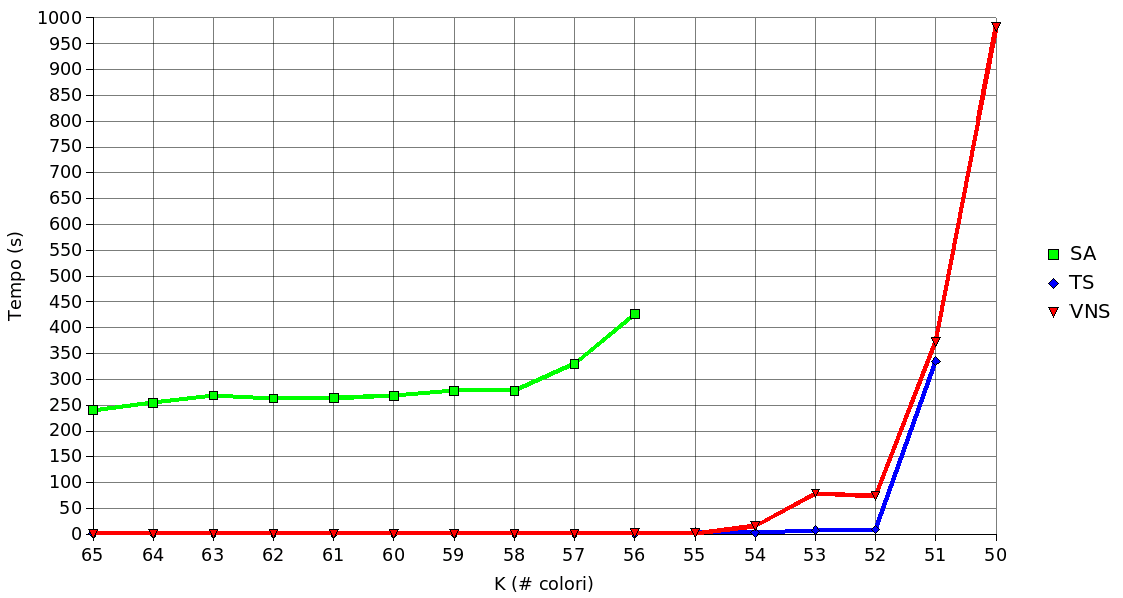
\includegraphics[width=0.5\textwidth,angle=-90]{img/500}
\caption[DSJC500: grafico colori-tempo]{Rappresentazione del tempo impiegato da parte delle tre differenti euristiche per la colorazione dell'istanza DSJC500.5 per numero di colori progressivamente decrescente. Si noti l'analogo andamento delle euristiche basate su ricerca locale e come invece si differenzia l'euristica di Simulated Annealing.}
\label{fig:500}
\end{center}
\end{figure}

\begin{figure}[h]
\begin{center}
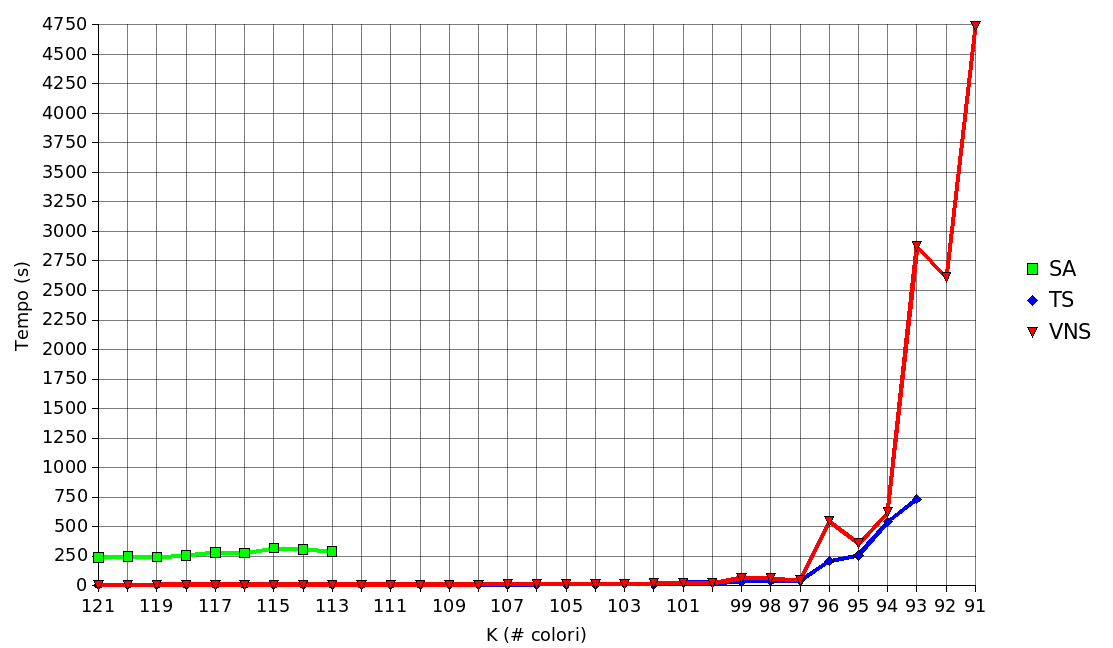
\includegraphics[width=0.5\textwidth,angle=-90]{img/1000}
\caption[DSJC1000: grafico colori-tempo]{Rappresentazione del tempo impiegato da parte delle tre differenti euristiche per la colorazione dell'istanza DSJC1000.5 per numero di colori progressivamente decrescente. Si noti anche in questo caso l'analogo andamento delle euristiche basate su ricerca locale e come invece si differenzia l'euristica di Simulated Annealing.}
\label{fig:1000}
\end{center}
\end{figure}

\clearpage
\begin{thebibliography}{}
\bibitem{tabucol}
Hertz A, de Werra D.
\emph{Using tabu search techniques for graph coloring.}
Computing 1987; 39:345--51.

\bibitem{tabusearch}
Glover F.
\emph{Future paths for integer programming and links to artificial intelligence.}
Computer and Operations Research 1986; 13/5:533--49.

\bibitem{tabucolimproved}
Galinier P, Hao J--K.
\emph{Hybrid evolutionary algorithms for graph coloring.}
Journal of Combinatorial Optimization 1999; 3:379--97.

\bibitem{sa}
Kirkpatrick S., Gelatt C. D., Vecchi M. P.
\emph{Optimization by Simulated Annealing.}
Science, 220: 671-680.

\bibitem{sa_metropolis}
Metropolis N., Rosenbaum A., Rosenbluth M, Teller A.
\emph{Equation of state calculations by fast computing machines.}
J. Chem. Phys. 21 (1953) 1087--1092.

\bibitem{sa_hertz_dewerra}
Chams M., Hertz A., de Werra D.
\emph{Some experiments with Simulated Annealing for coloring graphs.}
European Journal of Operational Research 32 (1987) 260--266.

\bibitem{sa_johnson}
Johnson D.S., Aragon C.R., McGeoch L.A., Shevon C.
\emph{Optimization by simulated annealing: an experimental evaluation; part II, graph coloring and number partitioning.}
Operations Research 1991; 39:378--406.

\bibitem{vns}
Mladenovic N., Hansen P.
\emph{Variable neighborhood search.}
Computers and Operations Research 1997; 24:1097--100.

\bibitem{vns_hertz}
Avanthay C., Hertz A., Zufferey N.
\emph{A variable neighborhood search for graph coloring.}
European Journal of Operational Research 2003; 151:379--88.

\bibitem{dimacs}
DIMACS graph coloring instances. \\
\emph{http://mat.gsia.cmu.edu/COLOR/instances.html}

\bibitem{survey}
Galinier P, Hertz A.
\emph{A survey of local search methods for graph coloring.}
Computer and Operations Research 2006; 33:2547--2562.
\end{thebibliography}

\end{document}
